\documentclass[12pt, twoside]{article}
\usepackage[letterpaper, margin=1in, headsep=0.5in]{geometry}
\usepackage[english]{babel}
\usepackage[utf8]{inputenc}
\usepackage{amsmath}
\usepackage{amsfonts}
\usepackage{amssymb}
\usepackage{tikz}
%\usetikzlibrary{quotes, angles}

\usepackage{graphicx}
\usepackage{enumitem}
\usepackage{multicol}

\usepackage{fancyhdr}
\pagestyle{fancy}
\fancyhf{}
\renewcommand{\headrulewidth}{0pt} % disable the underline of the header

\fancyhead[RE]{\thepage}
\fancyhead[RO]{\thepage \\ Name: \hspace{3cm}}
\fancyhead[L]{BECA / Dr. Huson / Geometry\\* 6 February 2019}

\begin{document}
\subsubsection*{7-6 Do Now: Quadratic graphs and transformations}
  \begin{enumerate}

\item Complete the t-chart for $x=0,1,2,3,4,5$, then graph and label the function on the grid below. Use pencil for graphs. Draw parabolas as smooth curves.

    \[f(x) = (x-3)^2-4\]


  \begin{center} %4 quadrant regents grid w T-Chart
  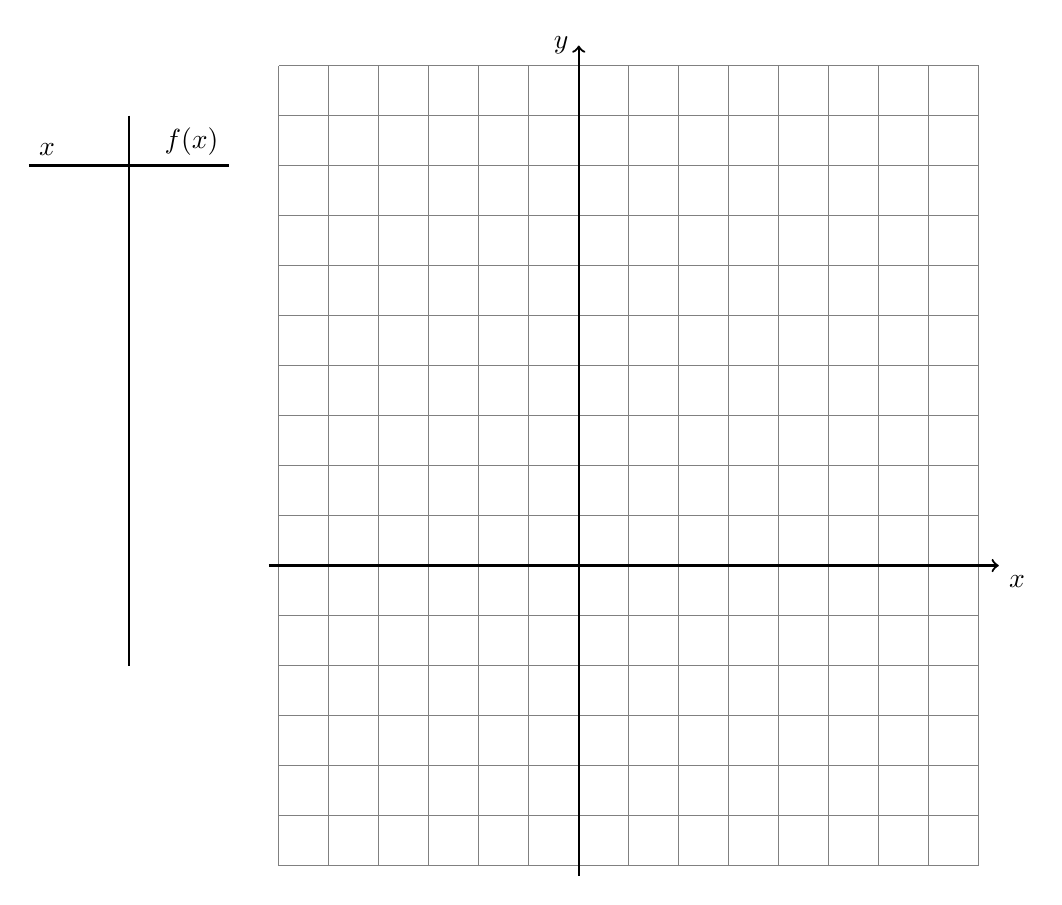
\begin{tikzpicture}[scale=.635]
    \draw [help lines] (-6,-6) grid (8,10);
    \draw [thick, ->] (-6.2,0) -- (8.4,0) node [below right] {$x$};
    \draw [thick, ->] (0,-6.2)--(0,10.4) node [left] {$y$};
    \draw [thick] (-11,8) node[above right]{$x$} --(-7,8) node [above left]{$f(x)$};
    \draw [thick] (-9,9)--(-9,-2);
  \end{tikzpicture}
  \end{center}

\begin{enumerate}
  \item Mark the vertex on the graph as an ordered pair.
  \item Write down the equation for the axis of symmetry. \vspace{2cm}
  \item The function is translated two units to the right and three units up, $f \rightarrow g$. What is the equation of $g$?
\end{enumerate}


\newpage

\item On the graph below, $\overleftrightarrow{AB}$ is shown with A(0, 6), B(9,0). A dilation of $k=\frac{2}{3}$ centered at the origin maps $\overleftrightarrow{AB} \rightarrow \overleftrightarrow{A'B'}$.\\*[0.5cm]
  Draw $\overleftrightarrow{A'B'}$ on the graph, labeling $A'$ and $B'$.
    \begin{center}
      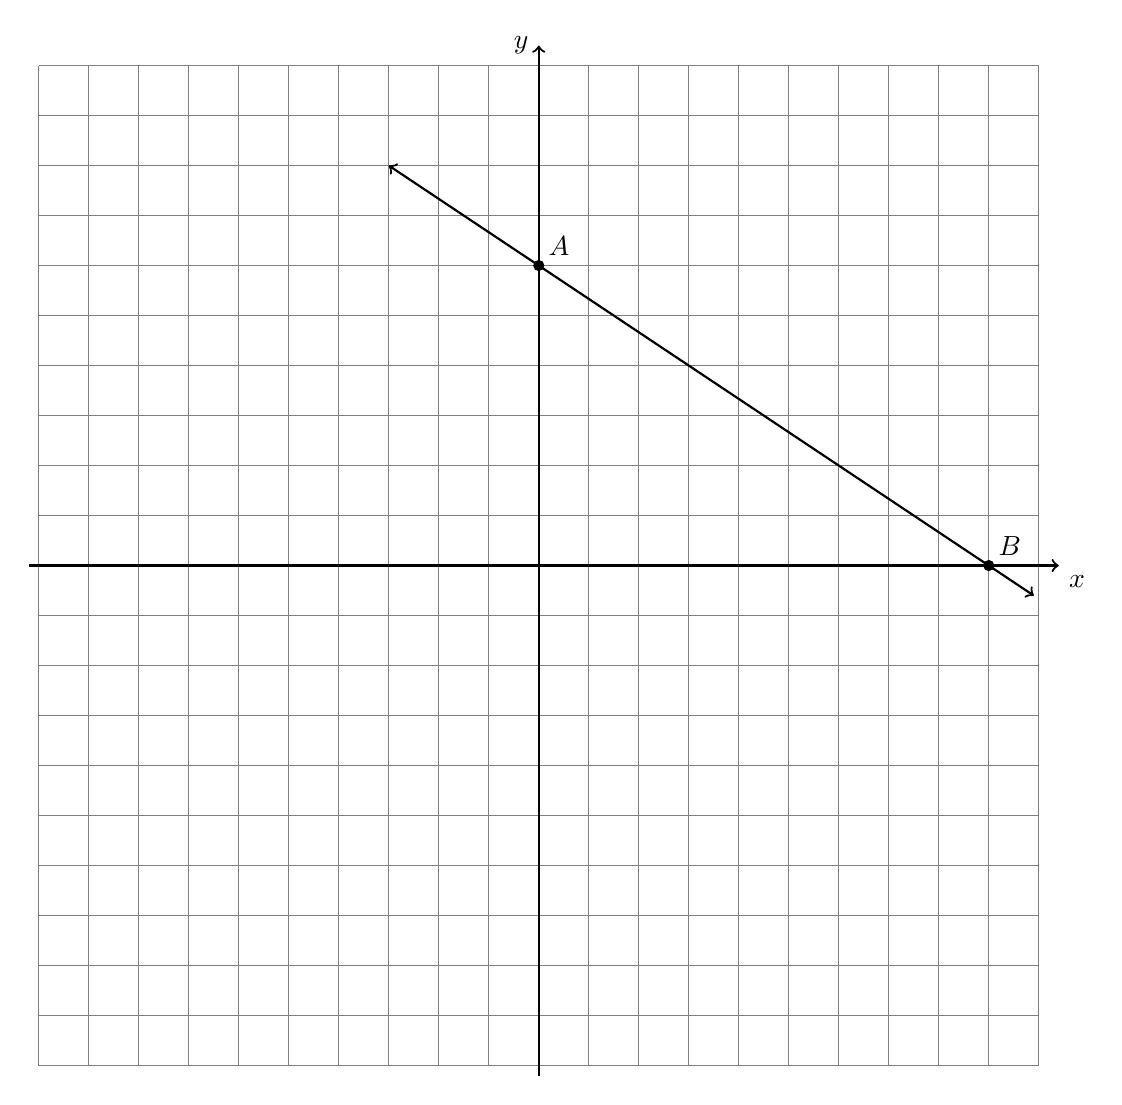
\begin{tikzpicture}[scale=.635]
        \draw [help lines] (-10,-10) grid (10,10);
        \draw [thick, ->] (-10.2,0) -- (10.4,0) node [below right] {$x$};
        \draw [thick, ->] (0,-10.2)--(0,10.4) node [left] {$y$};
        \draw [thick, <->] (-3,8)--(9.9,-0.6);
        \draw [fill] (0, 6) circle[radius = 0.1] node[above right]{$A$};
        \draw [fill] (9, 0) circle[radius = 0.1] node[above right]{$B$};
      \end{tikzpicture}
    \end{center}
      \vspace{1cm}
    \begin{enumerate}
      \item Write down the equation $\overleftrightarrow{AB}$ \vspace{2cm}
      \item Write down the equation $\overleftrightarrow{A'B'}$
    \end{enumerate}

\end{enumerate}

\end{document}
